\documentclass[]{article}
\usepackage{lmodern}
\usepackage{amssymb,amsmath}
\usepackage{ifxetex,ifluatex}
\usepackage{fixltx2e} % provides \textsubscript
\ifnum 0\ifxetex 1\fi\ifluatex 1\fi=0 % if pdftex
  \usepackage[T1]{fontenc}
  \usepackage[utf8]{inputenc}
\else % if luatex or xelatex
  \ifxetex
    \usepackage{mathspec}
  \else
    \usepackage{fontspec}
  \fi
  \defaultfontfeatures{Ligatures=TeX,Scale=MatchLowercase}
\fi
% use upquote if available, for straight quotes in verbatim environments
\IfFileExists{upquote.sty}{\usepackage{upquote}}{}
% use microtype if available
\IfFileExists{microtype.sty}{%
\usepackage{microtype}
\UseMicrotypeSet[protrusion]{basicmath} % disable protrusion for tt fonts
}{}
\usepackage[margin=1in]{geometry}
\usepackage{hyperref}
\hypersetup{unicode=true,
            pdftitle={Snow},
            pdfauthor={Kaisa Roggeveen, Scott Graham},
            pdfborder={0 0 0},
            breaklinks=true}
\urlstyle{same}  % don't use monospace font for urls
\usepackage{longtable,booktabs}
\usepackage{graphicx,grffile}
\makeatletter
\def\maxwidth{\ifdim\Gin@nat@width>\linewidth\linewidth\else\Gin@nat@width\fi}
\def\maxheight{\ifdim\Gin@nat@height>\textheight\textheight\else\Gin@nat@height\fi}
\makeatother
% Scale images if necessary, so that they will not overflow the page
% margins by default, and it is still possible to overwrite the defaults
% using explicit options in \includegraphics[width, height, ...]{}
\setkeys{Gin}{width=\maxwidth,height=\maxheight,keepaspectratio}
\IfFileExists{parskip.sty}{%
\usepackage{parskip}
}{% else
\setlength{\parindent}{0pt}
\setlength{\parskip}{6pt plus 2pt minus 1pt}
}
\setlength{\emergencystretch}{3em}  % prevent overfull lines
\providecommand{\tightlist}{%
  \setlength{\itemsep}{0pt}\setlength{\parskip}{0pt}}
\setcounter{secnumdepth}{0}
% Redefines (sub)paragraphs to behave more like sections
\ifx\paragraph\undefined\else
\let\oldparagraph\paragraph
\renewcommand{\paragraph}[1]{\oldparagraph{#1}\mbox{}}
\fi
\ifx\subparagraph\undefined\else
\let\oldsubparagraph\subparagraph
\renewcommand{\subparagraph}[1]{\oldsubparagraph{#1}\mbox{}}
\fi

%%% Use protect on footnotes to avoid problems with footnotes in titles
\let\rmarkdownfootnote\footnote%
\def\footnote{\protect\rmarkdownfootnote}

%%% Change title format to be more compact
\usepackage{titling}

% Create subtitle command for use in maketitle
\newcommand{\subtitle}[1]{
  \posttitle{
    \begin{center}\large#1\end{center}
    }
}

\setlength{\droptitle}{-2em}
  \title{Snow}
  \pretitle{\vspace{\droptitle}\centering\huge}
  \posttitle{\par}
  \author{Kaisa Roggeveen, Scott Graham}
  \preauthor{\centering\large\emph}
  \postauthor{\par}
  \predate{\centering\large\emph}
  \postdate{\par}
  \date{April 6th, 2018}

\newcommand{\Prob}{\operatorname{P}}
\newcommand{\E}{\operatorname{E}}
\newcommand{\Var}{\operatorname{Var}}
\newcommand{\Cov}{\operatorname{Cov}}
\newcommand{\se}{\operatorname{se}}
\newcommand{\re}{\operatorname{re}}
\newcommand{\ybar}{{\overline{Y}}}
\newcommand{\phat}{{\hat{p}}}
\newcommand{\that}{{\hat{T}}}
\newcommand{\med}{{\tilde{Y}}}
\newcommand{\logit}{{\operatorname{Logit}}}

\begin{document}
\maketitle

\section{Introduction}\label{introduction}

\subsection{Data}\label{data}

\begin{longtable}[]{@{}rrrrrrrrrrr@{}}
\caption{Wide Data}\tabularnewline
\toprule
Density & G 01 & G 02 & G 03 & G 04 & G 05 & G 06 & G 07 & G 08 & G 09 &
G 10\tabularnewline
\midrule
\endfirsthead
\toprule
Density & G 01 & G 02 & G 03 & G 04 & G 05 & G 06 & G 07 & G 08 & G 09 &
G 10\tabularnewline
\midrule
\endhead
0.686 & 17.6 & 17.3 & 16.9 & 16.2 & 17.1 & 18.5 & 18.7 & 17.4 & 18.6 &
16.8\tabularnewline
0.604 & 24.8 & 25.9 & 26.3 & 24.8 & 24.8 & 27.6 & 28.5 & 30.5 & 28.4 &
27.7\tabularnewline
0.508 & 39.4 & 37.6 & 38.1 & 37.7 & 36.3 & 38.7 & 39.4 & 38.8 & 39.2 &
40.3\tabularnewline
0.412 & 60.0 & 58.3 & 59.6 & 59.1 & 56.3 & 55.0 & 52.9 & 54.1 & 56.9 &
56.0\tabularnewline
0.318 & 87.0 & 92.7 & 90.5 & 85.8 & 87.5 & 88.3 & 91.6 & 88.2 & 88.6 &
84.7\tabularnewline
0.223 & 128.0 & 130.0 & 131.0 & 129.0 & 127.0 & 129.0 & 132.0 & 133.0 &
134.0 & 133.0\tabularnewline
0.148 & 199.0 & 204.0 & 199.0 & 207.0 & 200.0 & 200.0 & 205.0 & 202.0 &
199.0 & 199.0\tabularnewline
0.080 & 298.0 & 298.0 & 297.0 & 288.0 & 296.0 & 293.0 & 301.0 & 299.0 &
298.0 & 293.0\tabularnewline
0.001 & 423.0 & 421.0 & 422.0 & 428.0 & 436.0 & 427.0 & 426.0 & 428.0 &
427.0 & 429.0\tabularnewline
\bottomrule
\end{longtable}

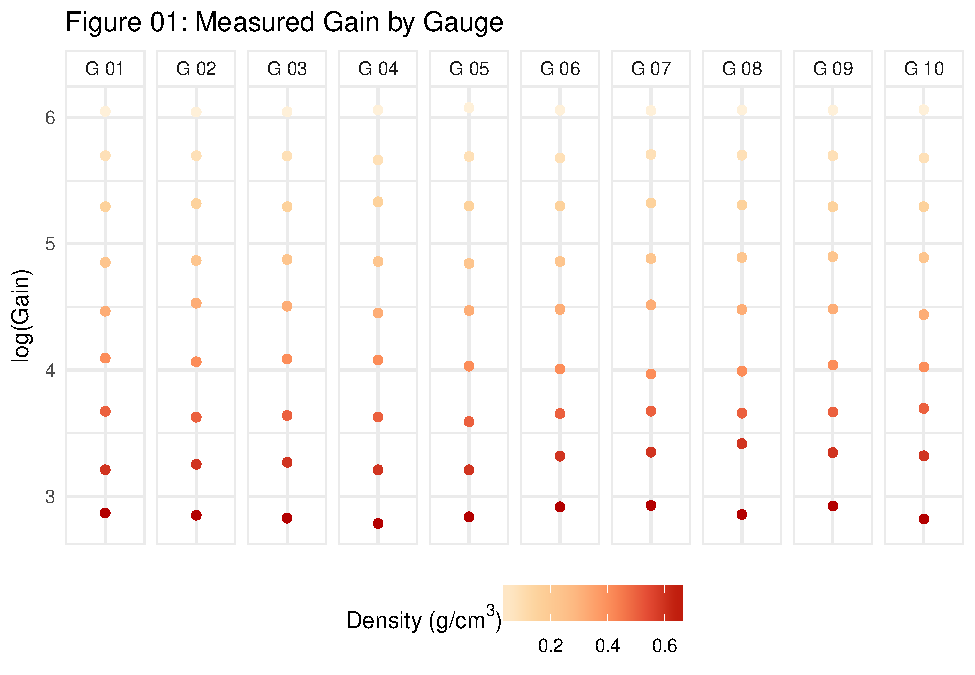
\includegraphics{Project_05_files/figure-latex/Measured Gain by Gauge-1.pdf}

Talk about how the gauges are consistent

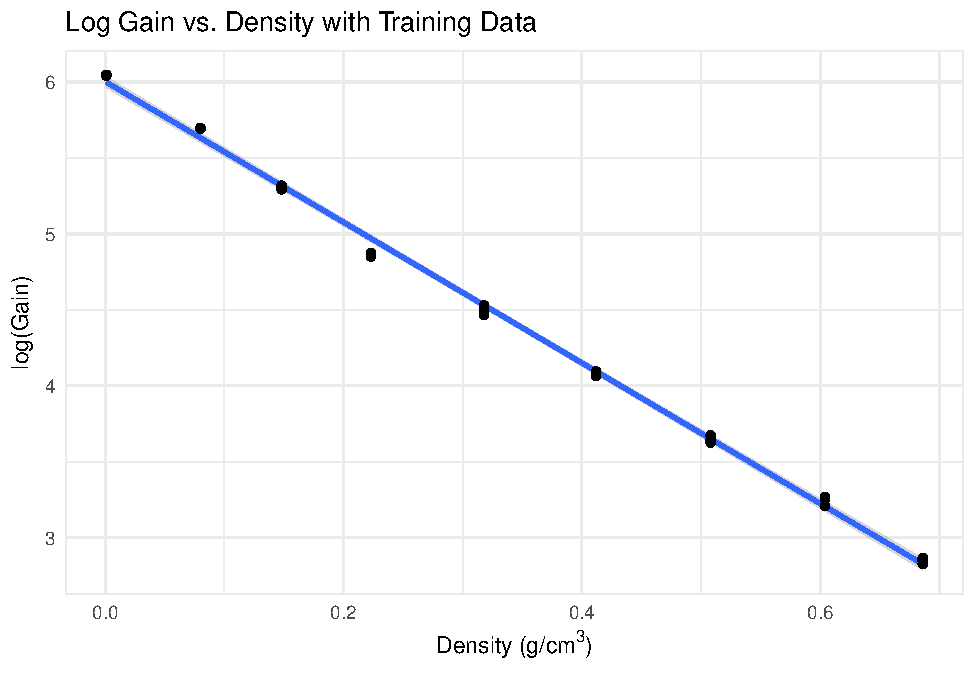
\includegraphics{Project_05_files/figure-latex/Training Data-1.pdf}

talk about how a log model is appropriate

\subsection{Training vs.~Validation
Data}\label{training-vs.validation-data}

Talk about how we split the data into training data (Gauges 1-3), and
validation data (gauges 4-10).

\section{Calibration}\label{calibration}

\subsection{Classic Calibration
Method}\label{classic-calibration-method}

For the classic calibration method, we regress our measurement (\(G:=\)
Gain) as a function of the known variable (\(D:=\) Density).

\begin{longtable}[]{@{}ccccc@{}}
\toprule
\begin{minipage}[b]{0.21\columnwidth}\centering\strut
~\strut
\end{minipage} & \begin{minipage}[b]{0.13\columnwidth}\centering\strut
Estimate\strut
\end{minipage} & \begin{minipage}[b]{0.16\columnwidth}\centering\strut
Std. Error\strut
\end{minipage} & \begin{minipage}[b]{0.12\columnwidth}\centering\strut
t value\strut
\end{minipage} & \begin{minipage}[b]{0.13\columnwidth}\centering\strut
Pr(\textgreater{}\textbar{}t\textbar{})\strut
\end{minipage}\tabularnewline
\midrule
\endhead
\begin{minipage}[t]{0.21\columnwidth}\centering\strut
\textbf{(Intercept)}\strut
\end{minipage} & \begin{minipage}[t]{0.13\columnwidth}\centering\strut
6.003\strut
\end{minipage} & \begin{minipage}[t]{0.16\columnwidth}\centering\strut
0.01799\strut
\end{minipage} & \begin{minipage}[t]{0.12\columnwidth}\centering\strut
333.6\strut
\end{minipage} & \begin{minipage}[t]{0.13\columnwidth}\centering\strut
3.897e-47\strut
\end{minipage}\tabularnewline
\begin{minipage}[t]{0.21\columnwidth}\centering\strut
\textbf{Density}\strut
\end{minipage} & \begin{minipage}[t]{0.13\columnwidth}\centering\strut
-4.63\strut
\end{minipage} & \begin{minipage}[t]{0.16\columnwidth}\centering\strut
0.04495\strut
\end{minipage} & \begin{minipage}[t]{0.12\columnwidth}\centering\strut
-103\strut
\end{minipage} & \begin{minipage}[t]{0.13\columnwidth}\centering\strut
2.182e-34\strut
\end{minipage}\tabularnewline
\bottomrule
\end{longtable}

\begin{longtable}[]{@{}cccc@{}}
\caption{Fitting linear model: log(Gain) \textasciitilde{}
Density}\tabularnewline
\toprule
\begin{minipage}[b]{0.18\columnwidth}\centering\strut
Observations\strut
\end{minipage} & \begin{minipage}[b]{0.27\columnwidth}\centering\strut
Residual Std. Error\strut
\end{minipage} & \begin{minipage}[b]{0.11\columnwidth}\centering\strut
\(R^2\)\strut
\end{minipage} & \begin{minipage}[b]{0.20\columnwidth}\centering\strut
Adjusted \(R^2\)\strut
\end{minipage}\tabularnewline
\midrule
\endfirsthead
\toprule
\begin{minipage}[b]{0.18\columnwidth}\centering\strut
Observations\strut
\end{minipage} & \begin{minipage}[b]{0.27\columnwidth}\centering\strut
Residual Std. Error\strut
\end{minipage} & \begin{minipage}[b]{0.11\columnwidth}\centering\strut
\(R^2\)\strut
\end{minipage} & \begin{minipage}[b]{0.20\columnwidth}\centering\strut
Adjusted \(R^2\)\strut
\end{minipage}\tabularnewline
\midrule
\endhead
\begin{minipage}[t]{0.18\columnwidth}\centering\strut
27\strut
\end{minipage} & \begin{minipage}[t]{0.27\columnwidth}\centering\strut
0.05255\strut
\end{minipage} & \begin{minipage}[t]{0.11\columnwidth}\centering\strut
0.9976\strut
\end{minipage} & \begin{minipage}[t]{0.20\columnwidth}\centering\strut
0.9976\strut
\end{minipage}\tabularnewline
\bottomrule
\end{longtable}

From this we take our linear regression model, and invert it, solving
for the known predictor variable \(D\). This gives us:

\[
  \hat{D_{i}} = 
  -\frac{\ln(G_{i}) - 6.0032 - \epsilon_{i}}{4.6301} =
  1.2965(1+\epsilon_{i}) - 0.2160\ln(G_{i}),
  \epsilon_{i} \stackrel{iid}{\sim} \mathcal{N}(0,\sigma^{2})
\]

From this, we can come up with both the point estimates for \(D\), and a
prediction interval, using: \[
  \se\left( \hat{D_{i}} \right) =
  \frac{\sqrt{MSE}}{\hat{\beta_{1}}}\sqrt{1 + \frac{1}{n} + \frac{\left( D_{i}-\bar{D} \right)^{2}}{S_{DD}}},
  MSE = 0.0028,
  \bar{D} = 0.3311\dots,
  S_{DD} = 0.2293
\]

As well as assuming an underlying Student's t-distribution, with
\(df=n-p=n-2=27-2=25\).

\begin{longtable}[]{@{}rrrrrr@{}}
\toprule
Density & Mean Gain & Est Density & Prediction Std. Error & Prediction
LB & Prediction UB\tabularnewline
\midrule
\endhead
0.001 & 428.71429 & -0.0124462 & 0.0141394 & -0.0415669 &
0.0166745\tabularnewline
0.080 & 295.42857 & 0.0679760 & 0.0131343 & 0.0409254 &
0.0950265\tabularnewline
0.148 & 201.71429 & 0.1503875 & 0.0123271 & 0.1249995 &
0.1757756\tabularnewline
0.223 & 131.00000 & 0.2436153 & 0.0117434 & 0.2194293 &
0.2678012\tabularnewline
0.318 & 87.81429 & 0.3300005 & 0.0115588 & 0.3061946 &
0.3538063\tabularnewline
0.412 & 55.75714 & 0.4281015 & 0.0117852 & 0.4038294 &
0.4523736\tabularnewline
0.508 & 38.62857 & 0.5073681 & 0.0122907 & 0.4820549 &
0.5326812\tabularnewline
0.604 & 27.47143 & 0.5809831 & 0.0129879 & 0.5542339 &
0.6077322\tabularnewline
0.686 & 17.61429 & 0.6769713 & 0.0141709 & 0.6477857 &
0.7061569\tabularnewline
\bottomrule
\end{longtable}

From this, we can plot the results, with the Estimated Density on the
y-axis, and the Mean Gain for a given Density on the x-axis. The grey
band represents the 95\% Prediction Interval for \(D\).

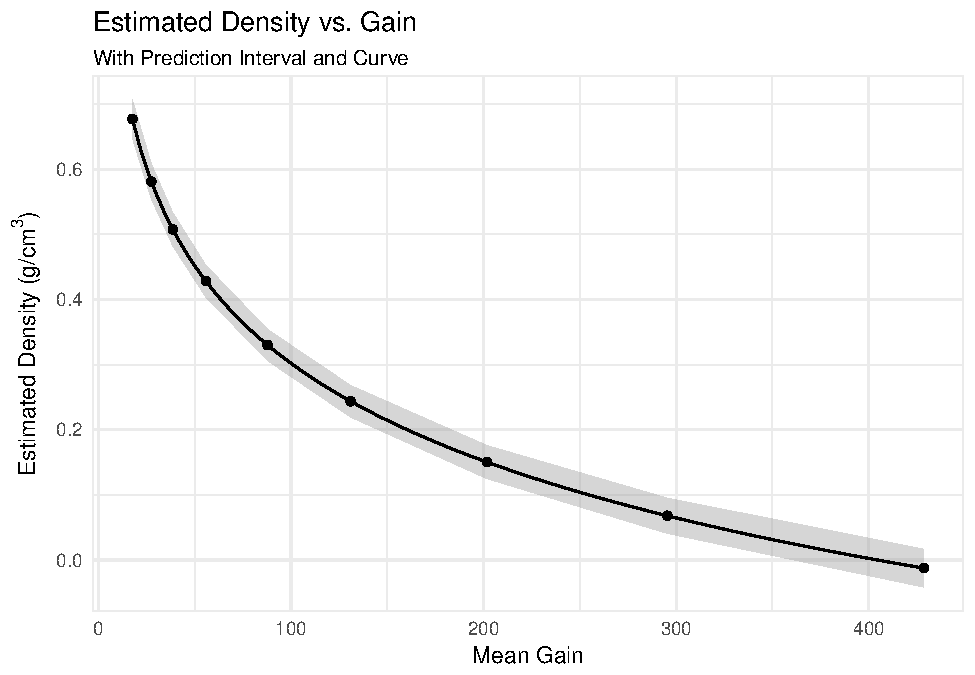
\includegraphics{Project_05_files/figure-latex/CC Dens vs Gain-1.pdf}

Parker et al. (2010), provides a method for finding a finding the bias
in the estimation of \(\hat{D_{i}}\): \[
  \operatorname{bias}\left( \hat{D_{i}} \right) =
  \frac{(D_{i} - \bar{D})MSE}{\hat{\beta_{1}}^{2}S_{DD}}
\]

\begin{longtable}[]{@{}rrrr@{}}
\caption{Unbiasing the Estimated Density for Classic
Calibration}\tabularnewline
\toprule
Density & Est Density & Bias & Unbiased Est Density\tabularnewline
\midrule
\endfirsthead
\toprule
Density & Est Density & Bias & Unbiased Est Density\tabularnewline
\midrule
\endhead
0.001 & -0.0124462 & -0.0001855 & -0.0122607\tabularnewline
0.080 & 0.0679760 & -0.0001411 & 0.0681171\tabularnewline
0.148 & 0.1503875 & -0.0001029 & 0.1504904\tabularnewline
0.223 & 0.2436153 & -0.0000607 & 0.2436760\tabularnewline
0.318 & 0.3300005 & -0.0000074 & 0.3300078\tabularnewline
0.412 & 0.4281015 & 0.0000454 & 0.4280560\tabularnewline
0.508 & 0.5073681 & 0.0000994 & 0.5072687\tabularnewline
0.604 & 0.5809831 & 0.0001533 & 0.5808297\tabularnewline
0.686 & 0.6769713 & 0.0001994 & 0.6767719\tabularnewline
\bottomrule
\end{longtable}

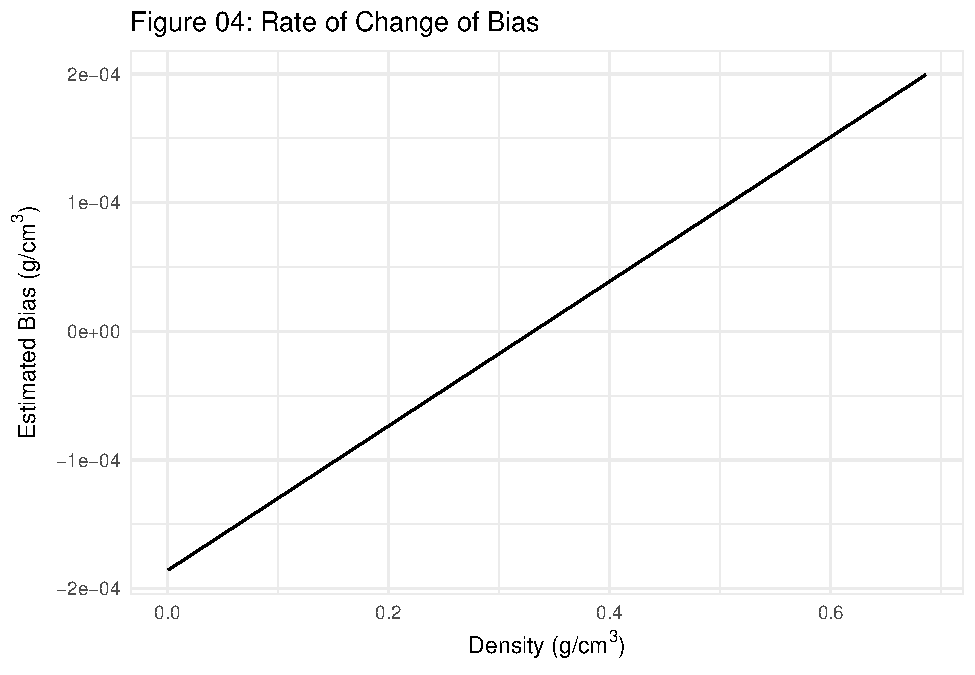
\includegraphics{Project_05_files/figure-latex/CC Unbias-1.pdf}

\subsection{Inverse Regression}\label{inverse-regression}

The other methodology looked at was using a inverse regression
technique, by using \(D\) as the dependent variable, and \(G\) as the
independent variable. This should give us a slightly different result
than the coefficients calculated under the classical calibration method,
as regression equations don't invert exactly unless the correlation
between the two variables is \(\pm 1\). Because our correlation
(-0.9061202) is close to \(-1\), the coefficients will be very close.
For this we use the model:

\[
  \hat{D_{i}} =
  \hat{\gamma_{0}} + \hat{\gamma_{1}}\left( \ln(G_{i}) - \overline{\ln(G_{i})} \right) + \epsilon_{i} =
  0.3311 - 02155\left( \ln(G_{i}) - 4.4701 \right) + \epsilon_{i},
  \epsilon_{i} \stackrel{iid}{\sim} \mathcal{N}(0,\sigma^{2})
\] \[
  \overline{\ln(G)} = \sum_{i=1}^{n}\frac{\ln{G_{i}}}{n},
  \hat{\gamma_{0}} = \bar{D}
\]

\begin{longtable}[]{@{}ccccc@{}}
\toprule
\begin{minipage}[b]{0.31\columnwidth}\centering\strut
~\strut
\end{minipage} & \begin{minipage}[b]{0.13\columnwidth}\centering\strut
Estimate\strut
\end{minipage} & \begin{minipage}[b]{0.16\columnwidth}\centering\strut
Std. Error\strut
\end{minipage} & \begin{minipage}[b]{0.12\columnwidth}\centering\strut
t value\strut
\end{minipage} & \begin{minipage}[b]{0.13\columnwidth}\centering\strut
Pr(\textgreater{}\textbar{}t\textbar{})\strut
\end{minipage}\tabularnewline
\midrule
\endhead
\begin{minipage}[t]{0.31\columnwidth}\centering\strut
\textbf{(Intercept)}\strut
\end{minipage} & \begin{minipage}[t]{0.13\columnwidth}\centering\strut
0.3311\strut
\end{minipage} & \begin{minipage}[t]{0.16\columnwidth}\centering\strut
0.002182\strut
\end{minipage} & \begin{minipage}[t]{0.12\columnwidth}\centering\strut
151.8\strut
\end{minipage} & \begin{minipage}[t]{0.13\columnwidth}\centering\strut
1.375e-38\strut
\end{minipage}\tabularnewline
\begin{minipage}[t]{0.31\columnwidth}\centering\strut
\textbf{log(\texttt{Centred\ Gain})}\strut
\end{minipage} & \begin{minipage}[t]{0.13\columnwidth}\centering\strut
-0.2155\strut
\end{minipage} & \begin{minipage}[t]{0.16\columnwidth}\centering\strut
0.002092\strut
\end{minipage} & \begin{minipage}[t]{0.12\columnwidth}\centering\strut
-103\strut
\end{minipage} & \begin{minipage}[t]{0.13\columnwidth}\centering\strut
2.182e-34\strut
\end{minipage}\tabularnewline
\bottomrule
\end{longtable}

\begin{longtable}[]{@{}cccc@{}}
\caption{Fitting linear model: Density \textasciitilde{}
log(\texttt{Centred\ Gain})}\tabularnewline
\toprule
\begin{minipage}[b]{0.18\columnwidth}\centering\strut
Observations\strut
\end{minipage} & \begin{minipage}[b]{0.27\columnwidth}\centering\strut
Residual Std. Error\strut
\end{minipage} & \begin{minipage}[b]{0.11\columnwidth}\centering\strut
\(R^2\)\strut
\end{minipage} & \begin{minipage}[b]{0.20\columnwidth}\centering\strut
Adjusted \(R^2\)\strut
\end{minipage}\tabularnewline
\midrule
\endfirsthead
\toprule
\begin{minipage}[b]{0.18\columnwidth}\centering\strut
Observations\strut
\end{minipage} & \begin{minipage}[b]{0.27\columnwidth}\centering\strut
Residual Std. Error\strut
\end{minipage} & \begin{minipage}[b]{0.11\columnwidth}\centering\strut
\(R^2\)\strut
\end{minipage} & \begin{minipage}[b]{0.20\columnwidth}\centering\strut
Adjusted \(R^2\)\strut
\end{minipage}\tabularnewline
\midrule
\endhead
\begin{minipage}[t]{0.18\columnwidth}\centering\strut
27\strut
\end{minipage} & \begin{minipage}[t]{0.27\columnwidth}\centering\strut
0.01134\strut
\end{minipage} & \begin{minipage}[t]{0.11\columnwidth}\centering\strut
0.9976\strut
\end{minipage} & \begin{minipage}[t]{0.20\columnwidth}\centering\strut
0.9976\strut
\end{minipage}\tabularnewline
\bottomrule
\end{longtable}

As we can see from the regression output,
\(\hat{\gamma_{0}} = \bar{D}\), which is what we want. We then estimated
\(\hat{D_{i}}\), and the prediction interval estimate:

\begin{longtable}[]{@{}rrrrrrr@{}}
\toprule
Density & Mean Gain & Mean Centred Gain & Est Density & Prediction Std.
Error & Prediction LB & Prediction UB\tabularnewline
\midrule
\endhead
0.001 & 428.71429 & 4.9072264 & -0.0116386 & 0.0209588 & -0.0548040 &
0.0315268\tabularnewline
0.080 & 295.42857 & 3.3815876 & 0.0685945 & 0.0176857 & 0.0321701 &
0.1050190\tabularnewline
0.148 & 201.71429 & 2.3088983 & 0.1508124 & 0.0147635 & 0.1204064 &
0.1812183\tabularnewline
0.223 & 131.00000 & 1.4994757 & 0.2438210 & 0.0123749 & 0.2183344 &
0.2693075\tabularnewline
0.318 & 87.81429 & 1.0051556 & 0.3300031 & 0.0115453 & 0.3062250 &
0.3537811\tabularnewline
0.412 & 55.75714 & 0.6382174 & 0.4278735 & 0.0125570 & 0.4020119 &
0.4537351\tabularnewline
0.508 & 38.62857 & 0.4421573 & 0.5069538 & 0.0146228 & 0.4768375 &
0.5370700\tabularnewline
0.604 & 27.47143 & 0.3144484 & 0.5803957 & 0.0171798 & 0.5450132 &
0.6157782\tabularnewline
0.686 & 17.61429 & 0.2016198 & 0.6761583 & 0.0210567 & 0.6327912 &
0.7195254\tabularnewline
\bottomrule
\end{longtable}

As well as recreating the plot used in the classical calibration method.
Note that the plot looks very similar, with a marginally large standard
error term.

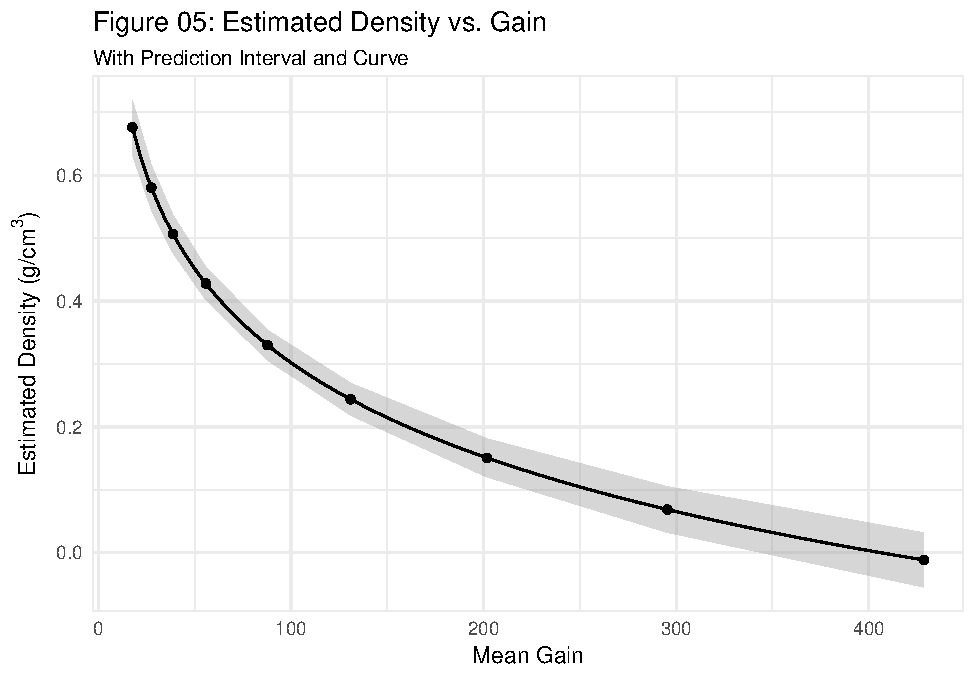
\includegraphics{Project_05_files/figure-latex/IR Dens vs Gain-1.pdf}

Parker et al. (2010), provides a means of unbiasing \(\hat{D_{i}}\) for
inverse regression too:

\[
  \operatorname{bias}\left( \hat{D_{i}} \right) =
  \frac{\bar{D} - D_{i}}{1 + \frac{\hat{\beta_{1}}^{2}S_{DD}}{(n-1)MSE}}
\]

This is then plotted against \(D\), to see the rate of change.

\begin{longtable}[]{@{}rrrr@{}}
\caption{Unbiasing the Estimated Density for Inverse
Regression}\tabularnewline
\toprule
Density & Est Density & Bias & Unbiased Est Density\tabularnewline
\midrule
\endfirsthead
\toprule
Density & Est Density & Bias & Unbiased Est Density\tabularnewline
\midrule
\endhead
0.001 & -0.0116386 & 0.0788687 & -0.0905073\tabularnewline
0.080 & 0.0685945 & 0.0599943 & 0.0086002\tabularnewline
0.148 & 0.1508124 & 0.0437481 & 0.1070643\tabularnewline
0.223 & 0.2438210 & 0.0258294 & 0.2179915\tabularnewline
0.318 & 0.3300031 & 0.0031324 & 0.3268706\tabularnewline
0.412 & 0.4278735 & -0.0193256 & 0.4471991\tabularnewline
0.508 & 0.5069538 & -0.0422615 & 0.5492153\tabularnewline
0.604 & 0.5803957 & -0.0651974 & 0.6455931\tabularnewline
0.686 & 0.6761583 & -0.0847885 & 0.7609467\tabularnewline
\bottomrule
\end{longtable}

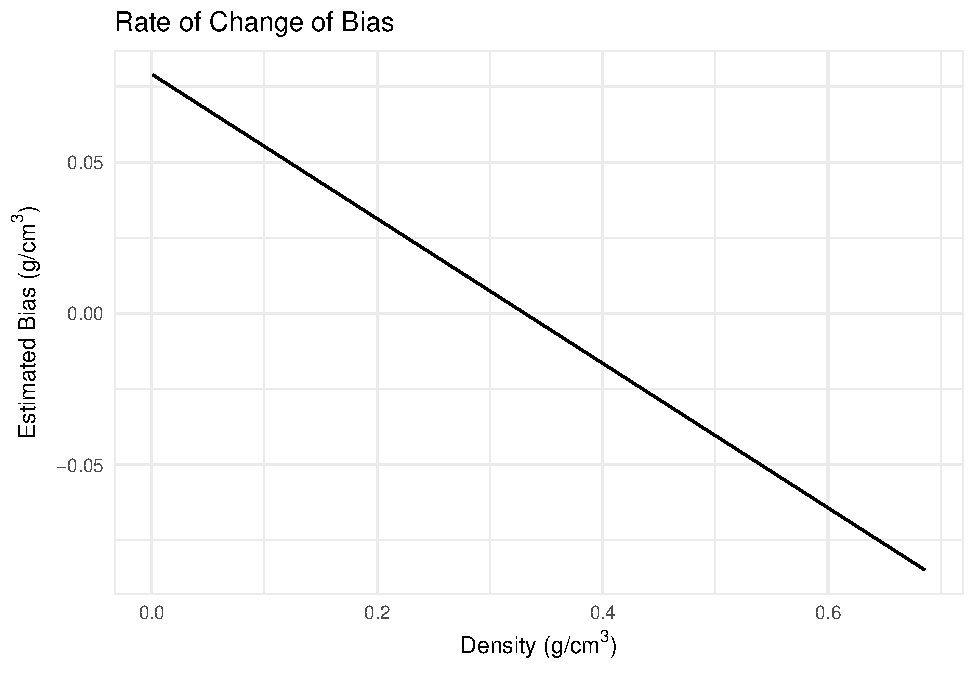
\includegraphics{Project_05_files/figure-latex/IR Unbias-1.pdf}

\subsection{Comparison}\label{comparison}

\begin{longtable}[]{@{}rrrrr@{}}
\caption{Comparison of Bias}\tabularnewline
\toprule
Density & CC Est Density & CC Bias & IR Est Density & IR
Bias\tabularnewline
\midrule
\endfirsthead
\toprule
Density & CC Est Density & CC Bias & IR Est Density & IR
Bias\tabularnewline
\midrule
\endhead
0.001 & -0.0124462 & -0.0001855 & -0.0116386 & 0.0788687\tabularnewline
0.080 & 0.0679760 & -0.0001411 & 0.0685945 & 0.0599943\tabularnewline
0.148 & 0.1503875 & -0.0001029 & 0.1508124 & 0.0437481\tabularnewline
0.223 & 0.2436153 & -0.0000607 & 0.2438210 & 0.0258294\tabularnewline
0.318 & 0.3300005 & -0.0000074 & 0.3300031 & 0.0031324\tabularnewline
0.412 & 0.4281015 & 0.0000454 & 0.4278735 & -0.0193256\tabularnewline
0.508 & 0.5073681 & 0.0000994 & 0.5069538 & -0.0422615\tabularnewline
0.604 & 0.5809831 & 0.0001533 & 0.5803957 & -0.0651974\tabularnewline
0.686 & 0.6769713 & 0.0001994 & 0.6761583 & -0.0847885\tabularnewline
\bottomrule
\end{longtable}

\begin{longtable}[]{@{}rrrrrr@{}}
\caption{Comparison of Standard Error}\tabularnewline
\toprule
Density & Mean Gain & CC Est Density & CC Prediction Std. Error & IR Est
Density & IR Prediction Std. Error\tabularnewline
\midrule
\endfirsthead
\toprule
Density & Mean Gain & CC Est Density & CC Prediction Std. Error & IR Est
Density & IR Prediction Std. Error\tabularnewline
\midrule
\endhead
0.001 & 428.71429 & -0.0124462 & 0.0141394 & -0.0116386 &
0.0209588\tabularnewline
0.080 & 295.42857 & 0.0679760 & 0.0131343 & 0.0685945 &
0.0176857\tabularnewline
0.148 & 201.71429 & 0.1503875 & 0.0123271 & 0.1508124 &
0.0147635\tabularnewline
0.223 & 131.00000 & 0.2436153 & 0.0117434 & 0.2438210 &
0.0123749\tabularnewline
0.318 & 87.81429 & 0.3300005 & 0.0115588 & 0.3300031 &
0.0115453\tabularnewline
0.412 & 55.75714 & 0.4281015 & 0.0117852 & 0.4278735 &
0.0125570\tabularnewline
0.508 & 38.62857 & 0.5073681 & 0.0122907 & 0.5069538 &
0.0146228\tabularnewline
0.604 & 27.47143 & 0.5809831 & 0.0129879 & 0.5803957 &
0.0171798\tabularnewline
0.686 & 17.61429 & 0.6769713 & 0.0141709 & 0.6761583 &
0.0210567\tabularnewline
\bottomrule
\end{longtable}

To compare the two methods, we looked at the size of their Bias, and the
size of the Standard Errors. From the two tables above, one can see that
the Classic Calibration method outperformed the Inverse Regression by
having both a smaller estimated bias, and a smaller estimated standard
error based on the same training and validation samples.

\subsection{Measurement Error}\label{measurement-error}

If we were to assume that the given densities for the polyethylene
blocks contained small amounts of measurement error, this change the
size of our interval estimates.

Let: \[
  \hat{D_{i}} =
  D_{i} + \epsilon_{D,i},
  \epsilon_{D,i} \sim \mathcal{N}(0, \sigma^{2}) \implies
\] \[
  \ln(G_{i}) = 
  \hat{\beta_{0}} + \hat{\beta_{1}}\hat{D_{i}} + \epsilon_{G,i} =
  \hat{\beta_{0}} + \hat{\beta_{1}}(D_{i} + \epsilon_{D,i}) + \epsilon_{G,i} =
\] \[
  \hat{\beta_{0}} + \hat{\beta_{1}}D_{i} + (\hat{\beta_{1}}\epsilon_{D,i} + \epsilon_{G,i}) =
  \hat{\beta_{0}} + \hat{\beta_{1}}D_{i} + \epsilon^{\star}_{G,i}
\] Where \[
  \epsilon^{\star}_{G,i} \sim
  \mathcal{N}\left( 0, \hat{\beta_{1}}^{2}\sigma_{D}^{2}+\sigma_{G}^{2}+2\hat{\beta_{1}}\Cov(D,G) \right)
\]

Now hopefully the covariance term is equal to 0, otherwise additional
issues would arise in the calibration. While this won't affect the
coefficient estimation done in the regressions, it would affect the size
of the interval estimates, by increasing them to reflect the greater
uncertainty in the quality of measurements.


\end{document}
